
\subsection{Prijem i rapoređivanje dostiglih namirnica}
\begin{figure}[h]
	\begin{center}
		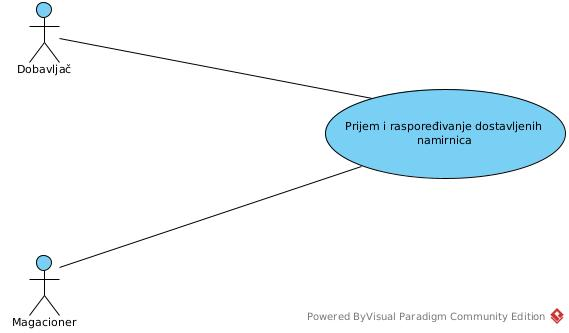
\includegraphics[scale=0.5]{uc_receiving_groceries}
	\end{center}
	\caption{Dijagram slučaja upotrebe prijema i raspoređivanja dostiglih namirnica}
\end{figure}
	\begin{itemize}
		\item{Kratak opis:} 
		
		- Magacioner prihvata dostigle namirnice i raspoređuje ih u magacinu
		\item{Učesnici:} 
		
		- Dobavljač, magacioner
		\item{Preduslovi:}
		
		- Magacioner i dobavljač su prijavljeni na sistem.
		\item{Postuslovi:}
		
		- Sve dostigle namirnice su raspoređene u magacinu i baza podataka je ažurirana.
		\item{Osnovni tok:}
		\begin{enumerate}
			\item{Dobavljač obaveštava magacionera o vremenu isporuke poručenih namirnica i njihovoj količini.}
			\item{Kamion sa poručenim namirnicama dolazi do magacina.}
			\item{Magacioner proverava spisak dostiglih namirnica i njihovu količinu sa listom poručenih namirnica:}
			\begin{enumerate}
			\item{Ako se spiskovi ne poklapaju, izvršava se podtok P1.}
			\end{enumerate}
			\item{Magacioner raspoređuje namirnice po magacinu.}
			\item{Magacioner obaveštava dobavljača da je završen prijem namirnica i šalje mu spisak primljenih namirnica.}
			\item{Dobavljač ažurira bazu podataka u skladu sa spiskom primljenih namirnica.}
		\end{enumerate}
		
		\item{Podtokovi:}
			\begin{enumerate}
				\item[P1.] \textbf{Spiskovi se ne poklapaju.} 
				\begin{enumerate}
				\item{Magacioner vrši evidenciju namirnica koje se ne poklapaju na spiskovima i kako se ne poklapaju.}
				\item{Magacioner preuzima samo namirnice koje se poklapaju na spiskovima i u potrebnoj količini ili manjoj.}
				\end{enumerate}
			\end{enumerate}
	\end{itemize}
\begin{figure}[h]
	\begin{center}
		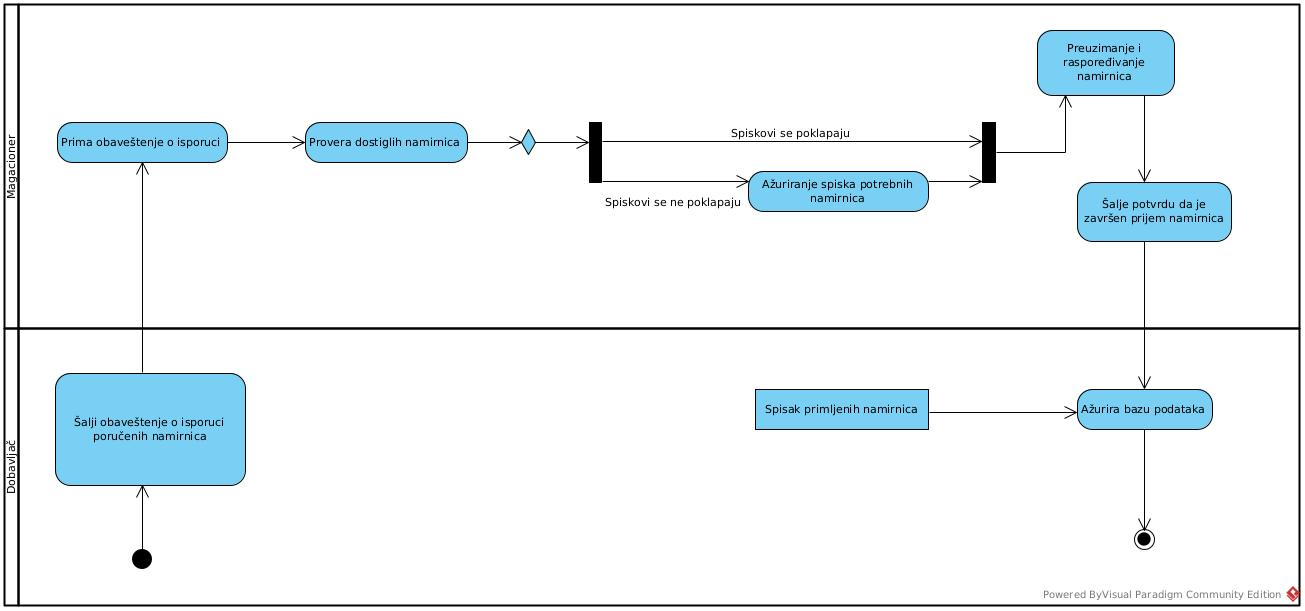
\includegraphics[width=\textwidth]{activity_receiving_groceries}
		\caption{Dijagram aktivnosti prijema i raspoređivanja dostiglih namirnica}
	\end{center}
\end{figure}
